\paragraph{QuizziPedia::Front-End::Controllers::LoginController}
\begin{figure} [ht]
	\centering
	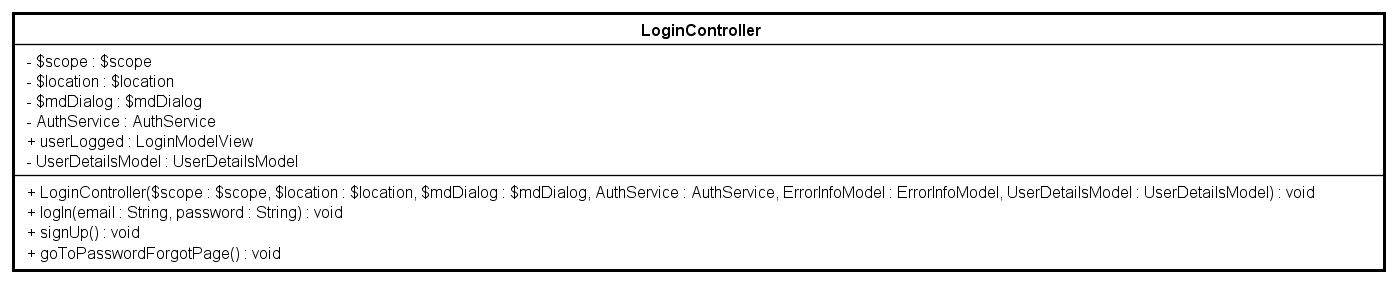
\includegraphics[scale=0.3]{UML/Classi/Front-End/QuizziPedia_Front-end_Controller_LoginController.png}
	\caption{QuizziPedia::Front-End::Controllers::LoginController}
\end{figure} \FloatBarrier
\begin{itemize}
	\item \textbf{Descrizione}: questa classe permette di gestire l'autenticazione dell'utente al sistema; 
	\item \textbf{Utilizzo}: fornisce le funzionalità di autenticazione al sistema, compresa la gestione di situazioni di errore di autenticazione;
	\item \textbf{Relazione con altre classi}:
	\begin{itemize}
		\item \textbf{IN} \texttt{LoginModelView}: classe di tipo modelview la cui istanziazione è contenuta all'interno della variabile di ambiente \$scope di \textit{Angular\ped{G}}. All'interno di essa sono presenti le variabili e i metodi necessari per il \textit{Two-Way Data-Binding\ped{G}} tra la \textit{view\ped{G}} \texttt{LoginView} e il \textit{controller\ped{G}} \texttt{LoginController};
		\item \textbf{IN} \texttt{AuthService}: questa classe permette di gestire la registrazione e l'autenticazione di un utente;
	\end{itemize}
	\item \textbf{Attributi}:
	\begin{itemize}
		\item \texttt{-} \texttt{\$scope: \$scope} \\
		Campo dati contenente un riferimento all’oggetto \$scope creato da \textit{Angular\ped{G}}. Viene utilizzato come mezzo di comunicazione tra il \textit{controller\ped{G}} e la \textit{view\ped{G}}. Contiene gli oggetti che definiscono il viewmodel e il \textit{model\ped{G}} dell’applicazione;
		\item \texttt{-} \texttt{\$location: \$location} \\
		Campo dati contenente un riferimento al servizio creato da \textit{Angular\ped{G}} che permette di accedere alla barra degli indirizzi del \textit{browser\ped{G}}, i cambiamenti all’URL nella barra degli indirizzi si riflettono in questo oggetto e viceversa;
		\item \texttt{-} \texttt{\$mdDialog: \$mdDialog} \\
		Campo dati contenente un riferimento al servizio della libreria \textit{Material for Angular\ped{G}} che permette di creare delle componenti a pop-up;
		\item \texttt{-} \texttt{AuthService: AuthService} \\
		Campo dati contenente un riferimento al servizio che si occupa della gestione delle informazioni legate all'autenticazione. Viene utilizzato il metodo \texttt{logIn()} di \$texttt{AuthService} a cui vengono passati i parametri \texttt{username} e \texttt{password};
		\item \texttt{+} \texttt{userLogged: UserDetailsModelView} \\
		Oggetto di tipo \texttt{UserDetailsModelView}. All'interno di essa sono presenti le variabili e i metodi necessari per il \textit{Two-Way Data-Binding\ped{G}} tra le \textit{views\ped{G}} e i \textit{controllers\ped{G}} che necessitano di utilizzare l'utente autenticato. Rappresenta nello \$rootScope un oggetto di tipo \texttt{UserDetailsModel}; \\
		\item \texttt{+} \texttt{UserDetailsModel: UserDetailsModel} \\
		Campo dati contenente un riferimento alla classe che rappresenta un utente. Contiene tutte le informazioni necessarie alla presentazione del contenuto di un utente sia nella visualizzazione che nella gestione di un profilo.
	\end{itemize}
	\item \textbf{Metodi}:
	\begin{itemize}
		\item \texttt{+} \texttt{LoginController(\$scope: \$scope, \$rootScope: \$rootScope, \$location:\\ \$location, \$mdDialog: \$mdDialog, AuthService: AuthService, ErrorInfoModel: ErrorInfoModel, UserDetailsModel: UserDetailsModel)} \\
		Metodo costruttore della classe. \\
		\textbf{Parametri}:
			\begin{itemize}
				\item \texttt{\$scope: \$scope} \\
				Parametro contenente un riferimento all’oggetto \$scope creato da \textit{Angular\ped{G}}. Viene utilizzato come mezzo di comunicazione tra il \textit{controller\ped{G}} e la \textit{view\ped{G}}. Contiene gli oggetti che definiscono il viewmodel e il \textit{model\ped{G}} dell'applicazione;
				\item \texttt{\$location: \$location} \\
				Parametro contenente un riferimento al servizio creato da \textit{Angular\ped{G}} che permette di accedere alla barra degli indirizzi del \textit{browser\ped{G}}, i cambiamenti all’URL nella barra degli indirizzi si riflettono in questo oggetto e viceversa;
				\item \texttt{\$mdDialog: \$mdDialog} \\
				Parametro contenente un riferimento al servizio della libreria \textit{Material for Angular\ped{G}} che permette di creare delle componenti a pop-up;
				\item \texttt{AuthService: AuthService} \\
				Parametro contenente un riferimento al servizio che si occupa della gestione delle informazioni legate all'autenticazione. Viene utilizzato il metodo \texttt{logIn()} di \$texttt{AuthService} a cui vengono passati i parametri \texttt{email} e \texttt{password};
				\item \texttt{ErrorInfoModel: ErrorInfoModel}: rappresenta le informazioni di un errore che si è verificato eseguendo una determinata operazione;
				\item \texttt{UserDetailsModel: UserDetailsModel} \\
				Parametro contenente un riferimento alla classe che rappresenta un utente. Contiene tutte le informazioni necessarie alla presentazione del contenuto di un utente sia nella visualizzazione che nella gestione di un profilo.
			\end{itemize}
		\item \texttt{+} \texttt{logIn(email: String, password: String): void} \\
		Metodo che richiama il metodo \texttt{signin} del service \texttt{AuthService} passandogli \texttt{email} e \texttt{password}. Nel caso di buona riuscita dell'operazione viene effettuato il redirect alla homepage dell'applicazione. Nel caso in cui invece avvenga un errore, viene mostrato a video il messaggio di errore;
		\item \texttt{+} \texttt{signUp(): void} \\
		Metodo che gestisce l'evento click sul pulsante di registrazione. Effettua il redirect alla pagina di registrazione;
		\item \texttt{+} \texttt{goToPasswordForgotPage(): void} \\
		Metodo che gestisce l'evento click sul pulsante di recupero password. Effettua il redirect alla pagina per il recupero della password.
	\end{itemize}
\end{itemize}

